\documentclass[final,hyperref={pdfpagelabels=false}]{beamer}
\mode<presentation>
{
  \usetheme{rc2018}
}
\usepackage[orientation=portrait,size=a0,scale=1.4,debug]{beamerposter}
\usepackage{siunitx}
%%%%%%%%%%%%%%%%%%%%%%%%%%%%%%%%%%%%%%%%%%%%%%%%%%%%%%%%%%%%%%%%%%%%%%%%%%%%%%%%% 5
\title{Influence of inhibitory circuits in the olfactory bulb on the frequency tuning of mitral cells}
\author[Miko]{Rebecca Miko, Christoph Metzner and Volker Steuber}
\institute{University of Hertfordshire, AL10 9AB, UK}
\date{Jul. 31th, 2018}

%%%%%%%%%%%%%%%%%%%%%%%%%%%%%%%%%%%%%%%%%%%%%%%%%%%%%%%%%%%%%%%%%%%%%%%%%%%%%%%%% 5
\begin{document}
\begin{frame}{} 
  \begin{block}{Motivation}
    The olfactory bulb (OB) in mammals is responsible for receiving, processing and relaying olfactory information (odours). 
    Naturalistic odour stimuli have a rich temporal structure, caused by turbulent airflow that mixes the odorant with clean air and other odorants. 
    Recent studies show that this structure contains information about the olfactory scene, for example the distance to an odour source $[1,2]$. 
    Furthermore, it has been suggested that animals might exploit this structure and extract this information in order to find odour sources $[3]$. 
    As some of this information may lie in the frequency content of the stimuli $[2]$, we studied input frequency dependent responses of mitral cells (MCs) in the olfactory bulb (OB), the first processing stage in the mammalian olfactory system.
    Specifically, we investigated whether MCs show frequency tuning and, if they do, how different components of the glomerular layer circuitry shape and determine the tuning.
  \end{block}

  \begin{columns}[t]
    \begin{column}{.48\linewidth}
      \begin{block}{Method} 
      	\begin{figure}
      		\center
      		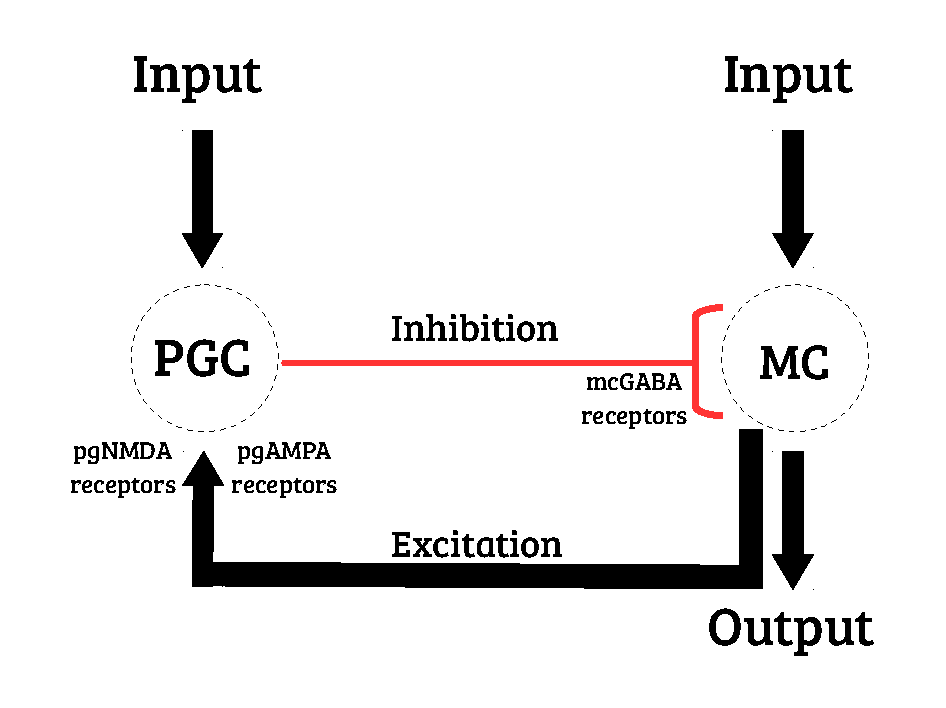
\includegraphics[scale=0.6]{images/Circuit_Diagram}
      		\end{figure}
      		\begin{itemize}
      			\item We used a model of the OB (modified from $[4]$) containing periglomerular cells (PGCs) and MCs.
      			\item The cell models have compartments, ion channels and synaptic receptors.
      			\item The synaptic conductances are modelled as double exponentials.
      			\item Postsynaptic currents were modelled using the equation from $[5]$.
      		\end{itemize}
      	      	
      	
      	
      		
      		
      	Using these cell models, a model of the MC - PGC motif was created, thus focusing on the recurrent and feed-forward inhibition in the glomerular layer, see Figure 1. 
      	The model records the membrane potential at the MC soma.
      	Simple sinusoidal currents of varying frequencies were used as input to the model, using the equation:
      	\begin{equation}
      	y(t) = csin(2 \pi ft + \varphi) + 0.18. 
      	\end{equation}
      	The phase $(\varphi)$ was always $0$. The strength of the input to the MC $(c)$ was $0.45nA$ for all simulations (run in NEURON), which defined the amplitude of the current, see Figure 2. 
      	
		\begin{figure}
      		\center
      		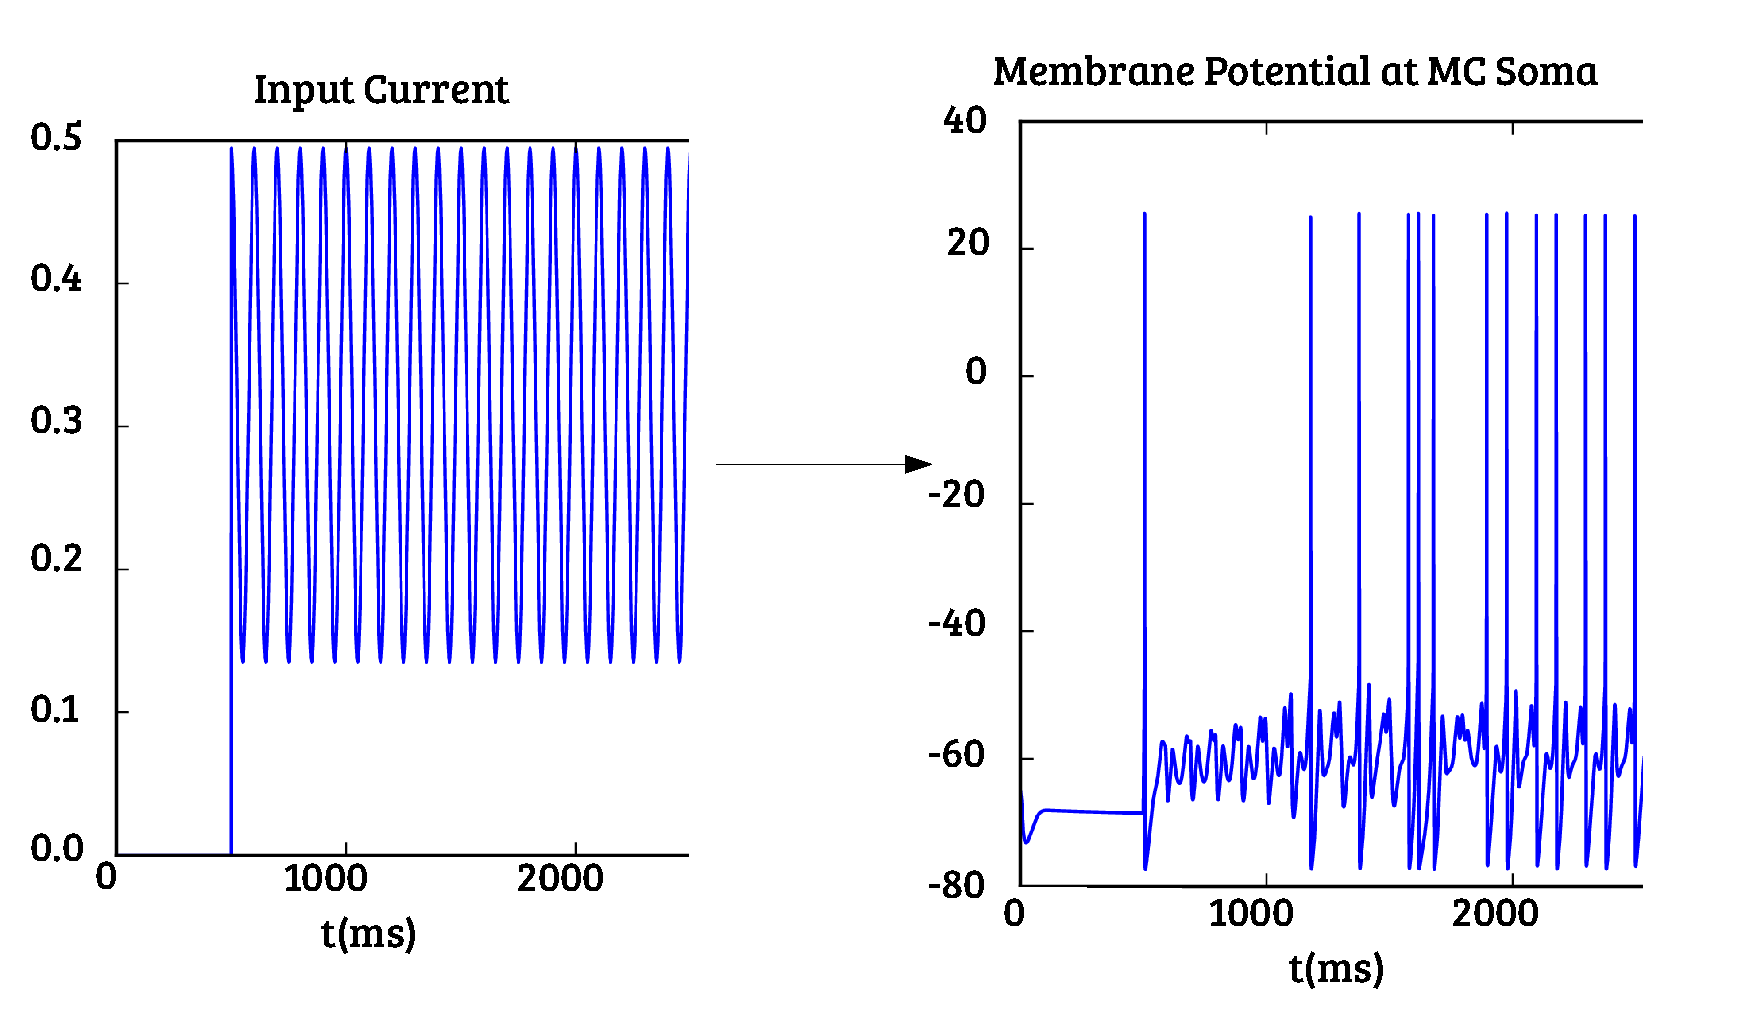
\includegraphics[scale=1.2]{images/Figure2}
      		\end{figure} 
      		
      	The PGC input strength was adjusted by multiplying $0.45nA$ by the values: $0.2, 0.3, 0.4, 0.5$ and $0.6$. 
      	The MC - PGC excitation strength varied using $W_{exc}$ values: $2.0, 4.0, 6.0, 8.0$ and $10.0$. 
      	Finally, the PGC - MC inhibition strength varied using $W_{inh}$ values: $1.0, 2.0, 3.0, 4.0$ and $5.0$. 
		The frequency $(f)$ of the input ranged between 
		%\SI{1.0}{\hertz}
		%$1.0\mathrm{~}Hz$
		%\num{1.0}~Hz\\
		1.0Hz
		and $40.0Hz$ (with a step size of $1.0$). 
		The output from the MC was recorded and from this the firing rates were calculated. 
		For each parameter combination (PGC input strength, MC - PGC excitation strength, PGC - MC inhibition strength) we constructed frequency tuning curves by plotting firing rate against input frequency, see Figure 3. 
		From these tuning curves we extracted the peakresonance frequency and the strength of the tuning $Q$, which was measured as:
		\begin{equation}
		Q = \frac{(F_{max} - F_{min})}{<F>}
		\end{equation}
		where $F_{max}$ and $F_{min}$ is the maximum and minimum firing rate, and $<F>$ is the mean firing rate over all measured frequencies. Figure 4 summarises the results.
      \end{block}
    \end{column}
    \begin{column}{.48\linewidth}
      \begin{block}{Results}
      	\begin{figure}
      		\center
      		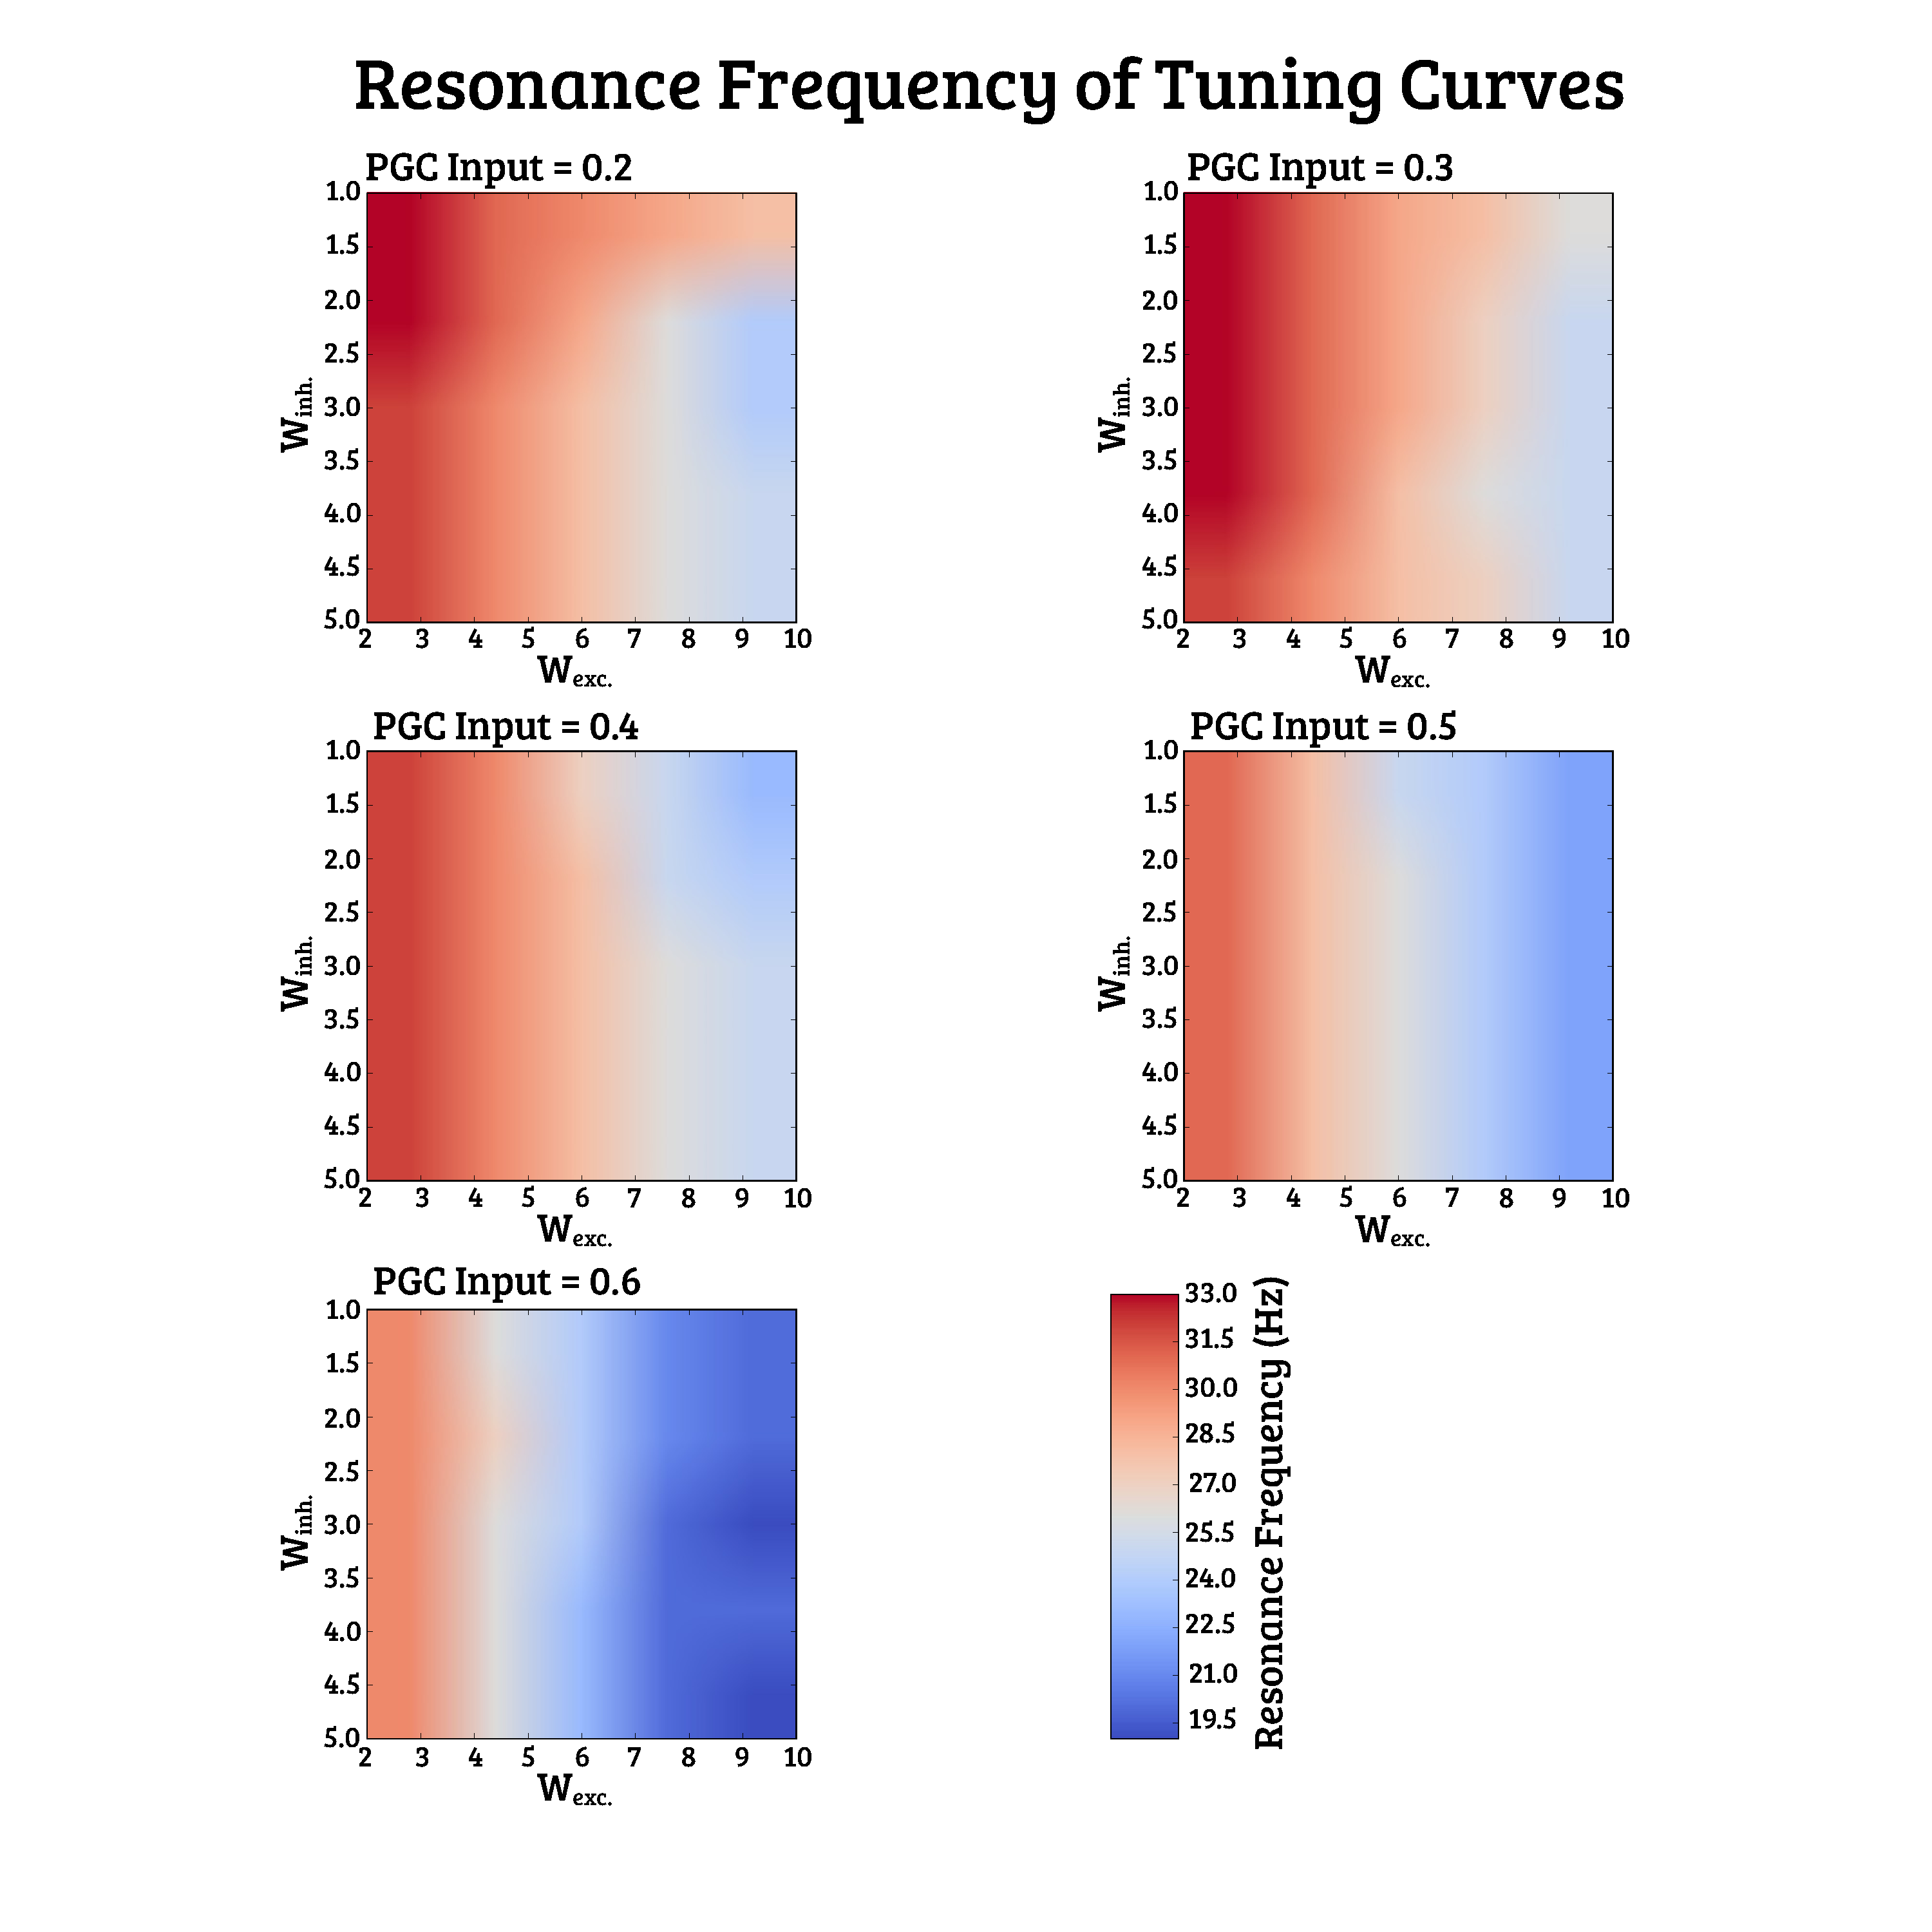
\includegraphics[scale=0.5]{images/Contour_plot_tuning_frequency}
      		\end{figure} 
        We found that the resonance frequency decreased as the excitation of the PGC (both from the input and from the MC) increased, whereas the strength of the PGC inhibition onto the MC did not seem to have a strong effect. 
        Furthermore, the resonance strength increased with the strength of the excitatory connection between the MC and the PGC when the PGC received sufficient external input from olfactory stimuli.
      \end{block}

      \begin{block}{Discussion}
      	\begin{figure}
      		\center
      		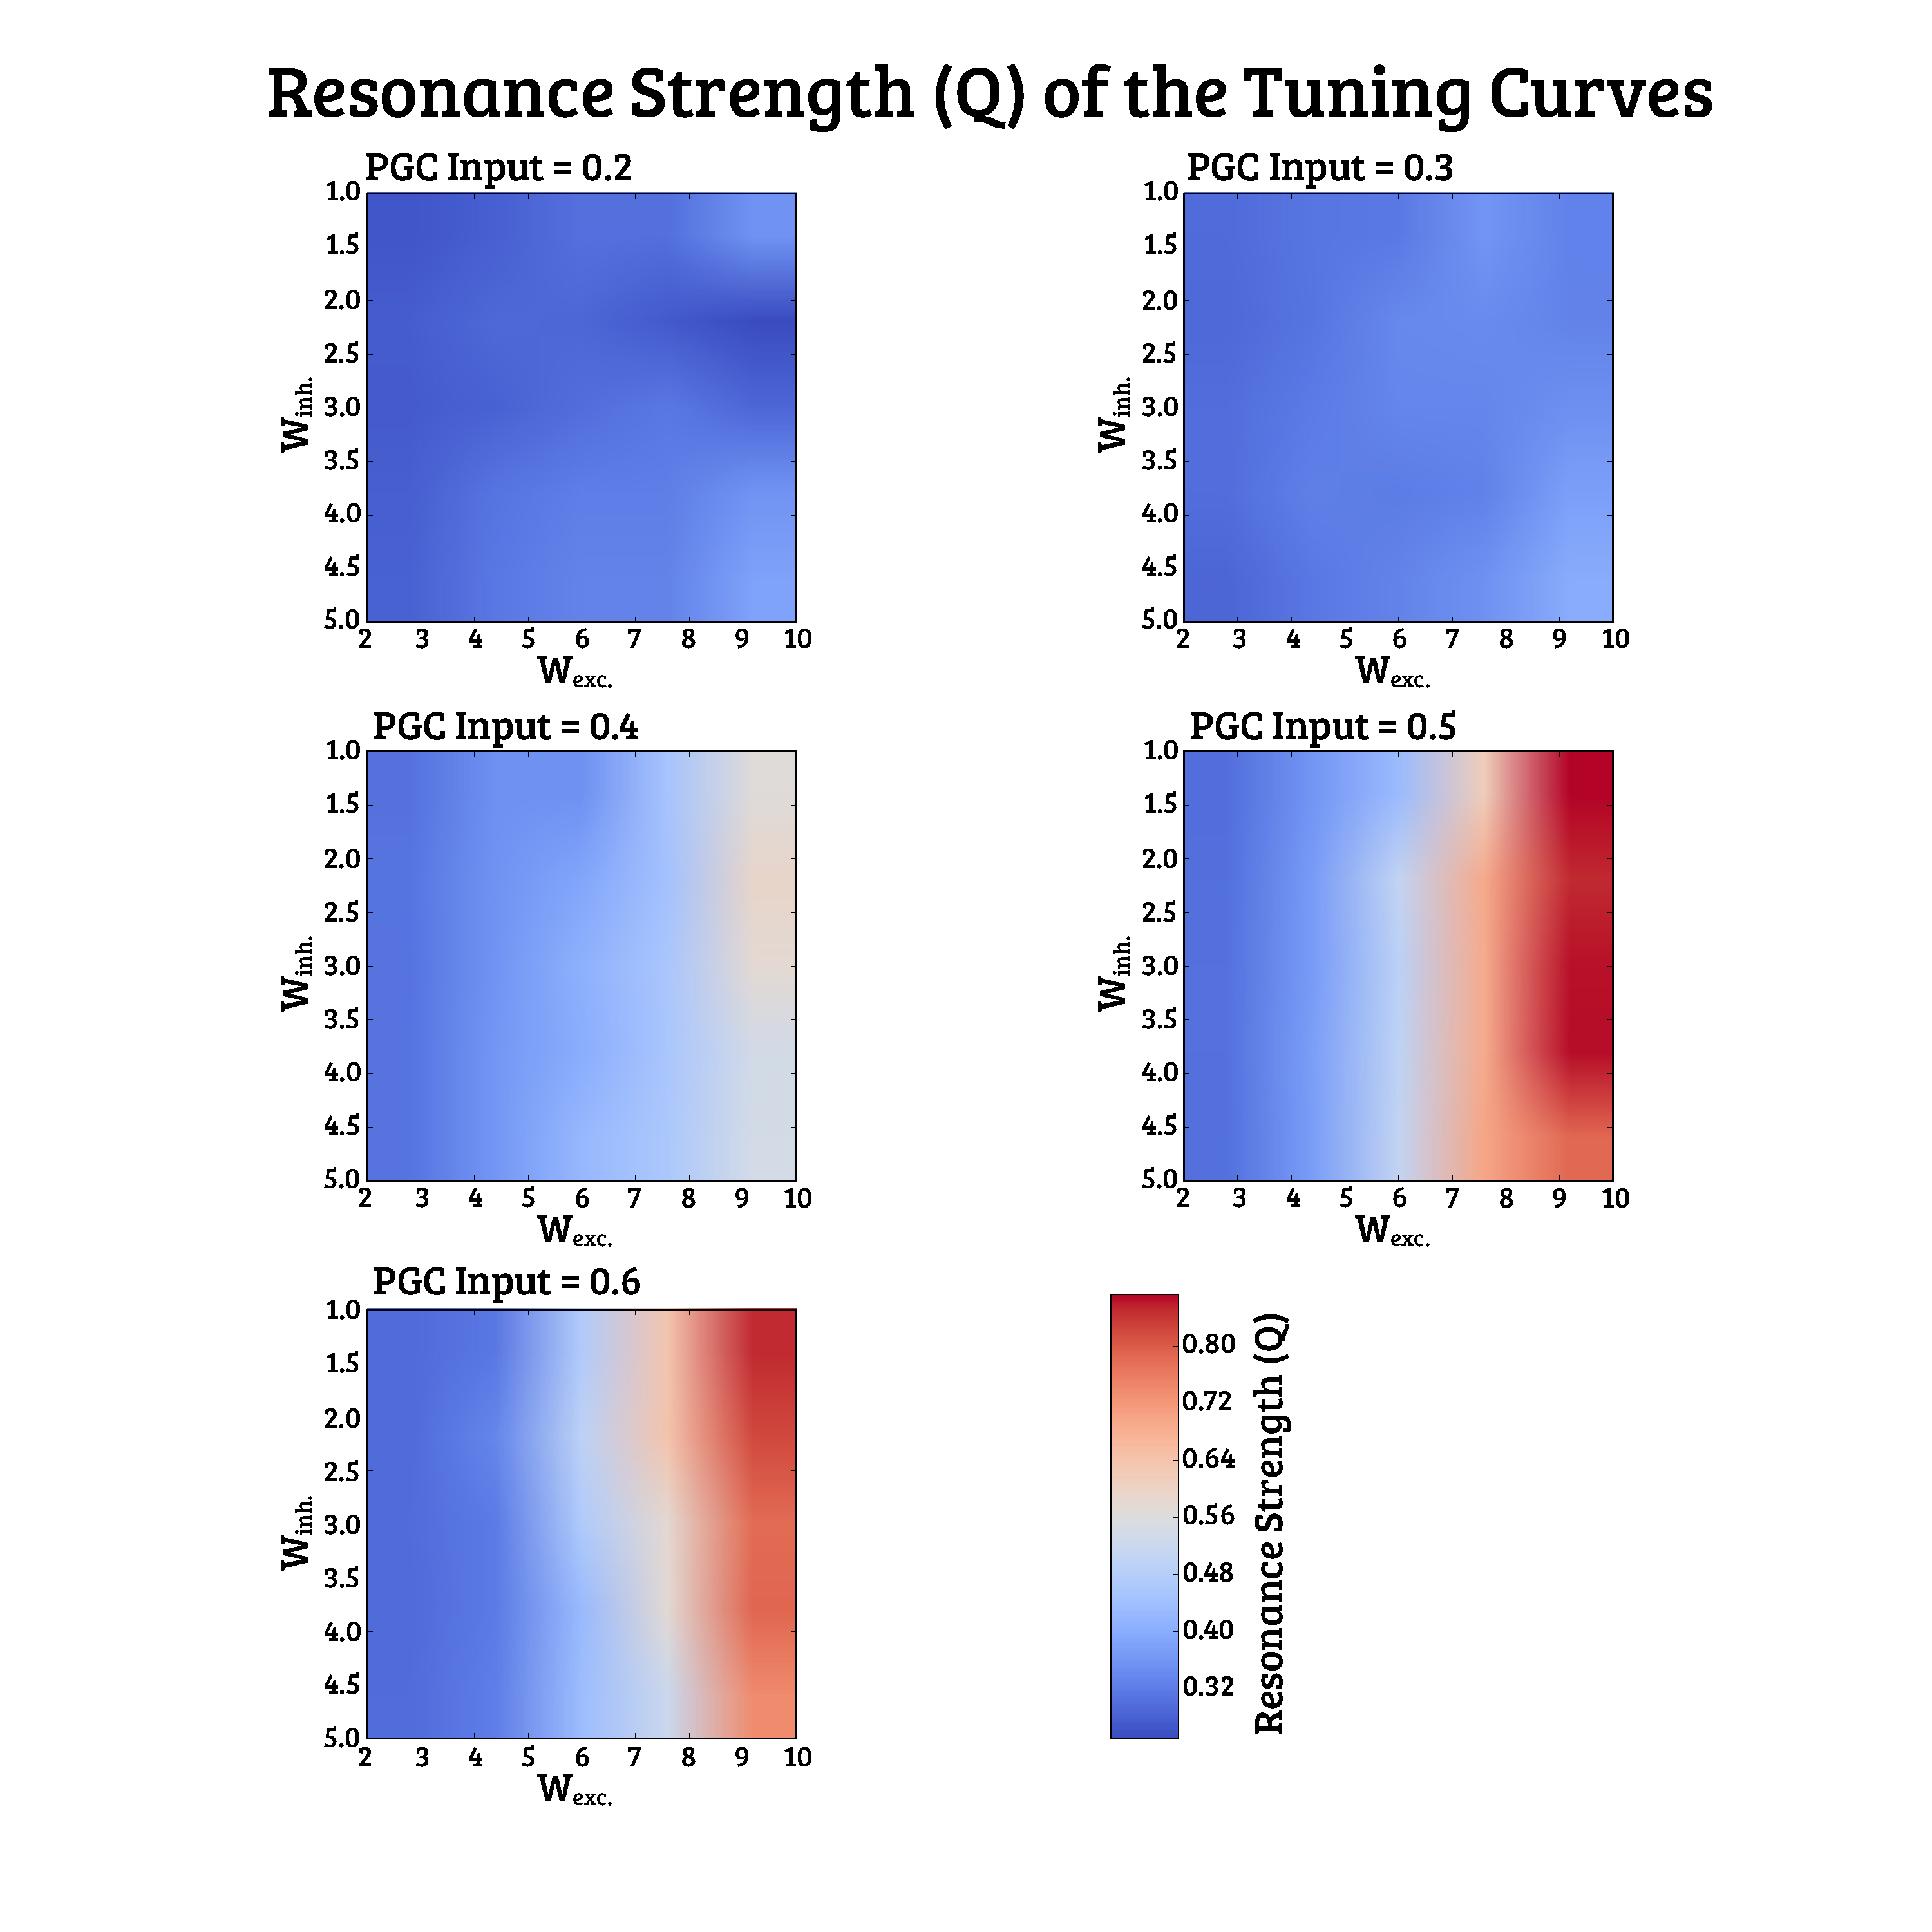
\includegraphics[scale=0.5]{images/Contour_plot_tuning_strength}
      		\end{figure} 
        These results suggest that the MC can indeed show frequency tuning and that this depends on the strength of the excitatory synaptic input to the PGC, which provide inhibitory input to the MC.
        However, the observed frequency tuning occurred in a narrow range ($19.5Hz – 33.0Hz$).
        Future work should investigate how the OB could use this frequency tuning to obtain information about the surrounding olfactory scene.
      \end{block}
    \end{column}
  \end{columns}
\end{frame}
\end{document}

%%%%%%%%%%%%%%%%%%%%%%%%%%%%%%%%%%%%%%%%%%%%%%%%%%%%%%%%%%%%%%%%%%%%%%%%%%%%%%%%%%%%%%%%%%%%%%%%%%%% 
%%% Local Variables: 
%%% mode: latex
%%% TeX-engine: xetex
%%% End: